


How can we reduce traffic congestion? Can we structure our road networks so that navigation is both fast and the impact on the environment is reduced? In this section, we investigate these questions trying to provide answers based on our traffic emulator.

We are interested in finding the optimal parameters' configuration in order to minimise our outputs. However, the function we aim to optimise is explicitly unknown and querying it for a single data point takes a few seconds. For this reason, we use Bayesian Optimisation (BO), already introduced in section \ref{sec:bo_background}. In this work, we choose Expected Improvement as our acquisition function. Optimisation is ran on the models acquired from experimental design (\ref{sec:experimental-design}).

The resulting optimal points can be seen in Table \ref{table:optimal_points}. We observe that for both models the lowest output is found with minimum speed and maximum road length. Intuitively, navigating networks with shorter roads implies spending more time traversing intersections, which are a major source of delay and pollution in cities. The low speed limit benefits emissions as it implies that less trip time will be spent accelerating. We also see that more lanes benefit time loss while fewer lanes are better to optimise emissions. This is intuitive as lane changes are known to increase pollution \cite{rakha2000requirements}. Finally, the optimal acceleration to optimise emissions may be an unexpected result, but we know that a vehicle's emission efficiency curve is never zero. Thus, a lengthy, low acceleration trip may emit more CO$_2$ than a short, erratic one.

\begin{table}[h!]
    \centering
    \caption{Optimal parameters' configurations found with Bayesian Optimisation}
    \label{table:optimal_points}
    \begin{tabular}{@{} l *5c l c @{} }
    \toprule
    \multicolumn{1}{c}{Emulator}  & $N_G$ &  $v_{max}$ & $L_E$ & $N_L$ & $\alpha_V$ & Output \\ 
    \midrule
        Time loss & 10 & 8 & 70 & 2 & 1.86 & 12.37\\
        Emissions & 20 & 8 & 61.36 & 1 & 2.96 & 1721.50\\
    \midrule
        Average & 15 & 8 & 65.68 & 1 & 2.28 & \\
    \bottomrule
    \end{tabular}
\end{table}

We investigate more deeply the grid size. We observe that the two models pick very different grid size values, this suggests that there could be a trade-off related to the grid size and that optimising this size for both objectives is pareto-optimal. For this purpose, we analyse the simulator and the emulators in the average optimal point shown in Table \ref{table:optimal_points}.
In Figure~\ref{fig:trade_off} we observe that indeed this trade-off exists in the simulator and our emulators are able to capture it. This gives insights on the fact that when planning urban areas the size of the network is a crucial factor. Choices that benefit travel time may pose a danger for the environment.

\begin{figure}[b!]
\centering
\begin{subfigure}{0.5\textwidth}
  \centering
  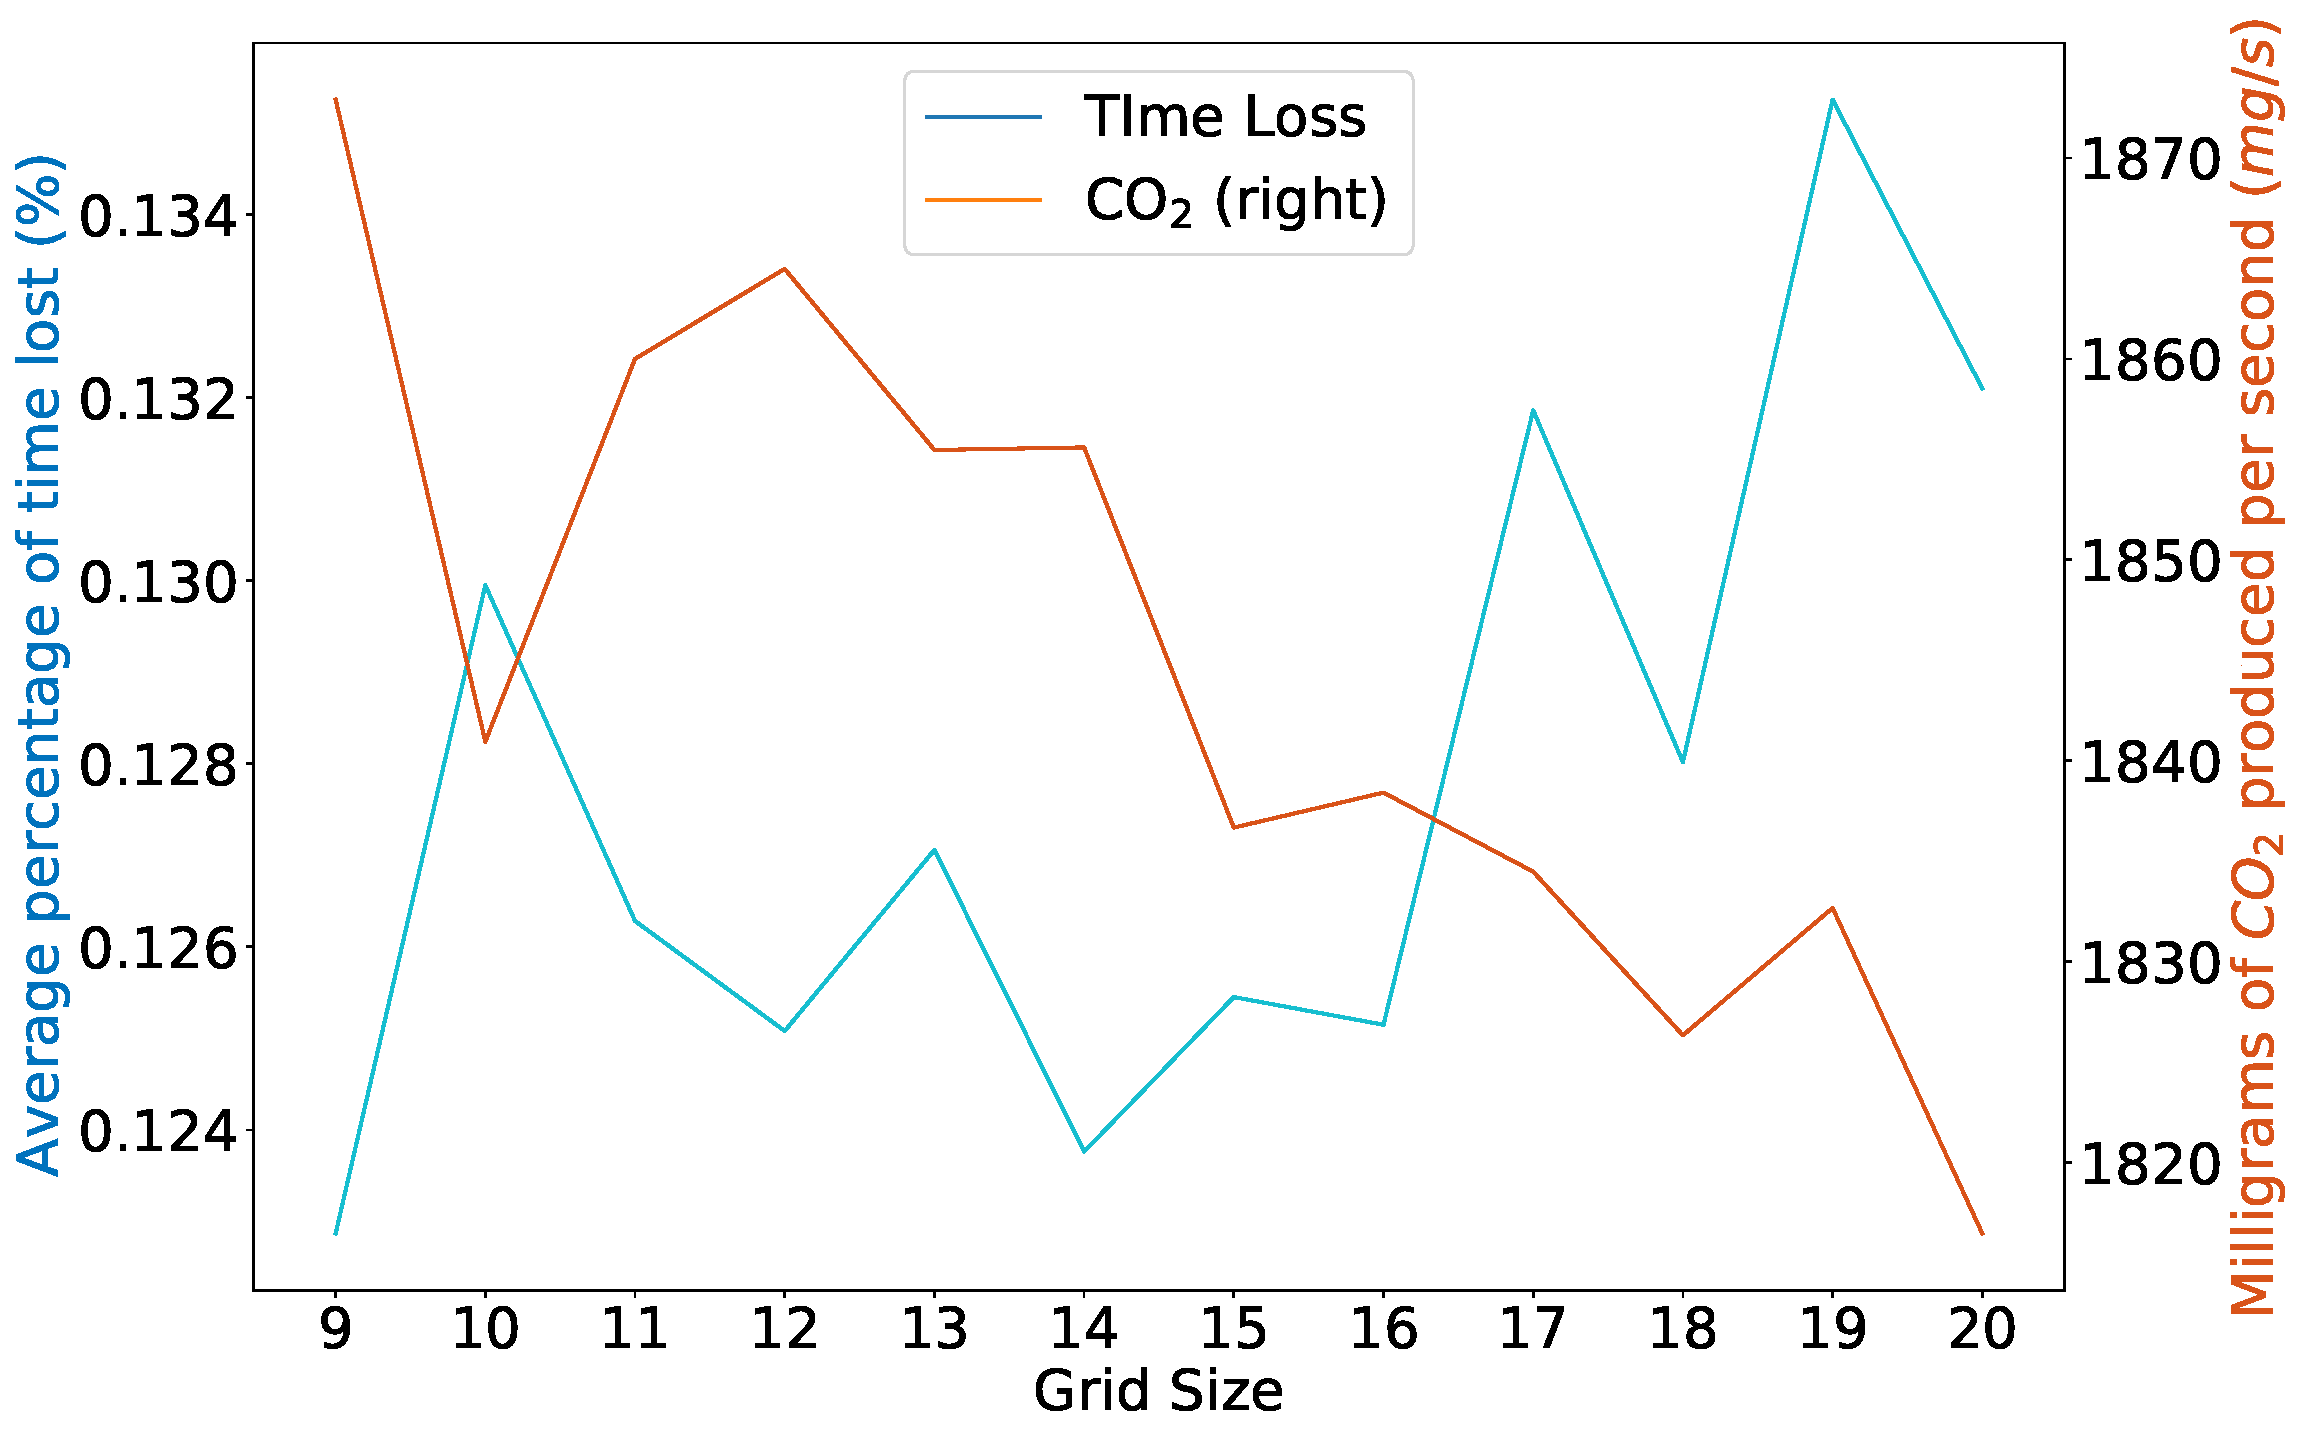
\includegraphics[width=\textwidth]{trade-off_simulator_gridSize}
  \caption{Simulator}
\end{subfigure}%
\begin{subfigure}{0.5\textwidth}
  \centering
  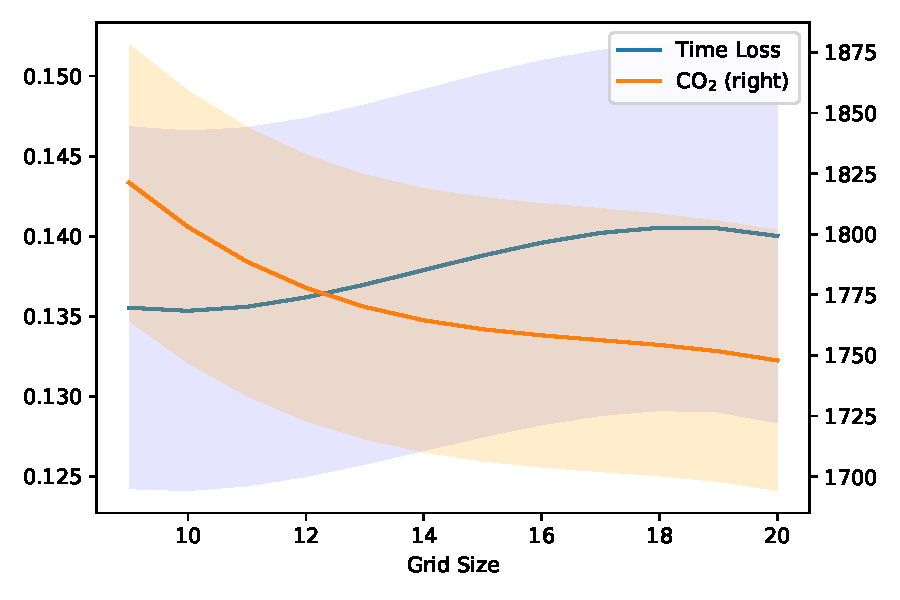
\includegraphics[width=\textwidth]{small_grid_size}
  \caption{Emulator}
\end{subfigure}
\caption{Trade-off between CO$_2$ and time loss when varying the grid size in the average optimal point}
\label{fig:trade_off}
\end{figure}

Finally, as we run Bayesian optimisation on the experimentally designed emulators, we aim to compare the difference between the emulators before and after the optimisation phase. In Figure~\ref{fig:grid_size_comp} we see that for grid size the predictive variance decreases significantly and also the prediction mean is subject to modification. For further comparisons please refer to Appendix~\ref{appendix:comparison}.

\begin{figure}[t!]
\centering
\begin{subfigure}{0.5\textwidth}
  \centering
  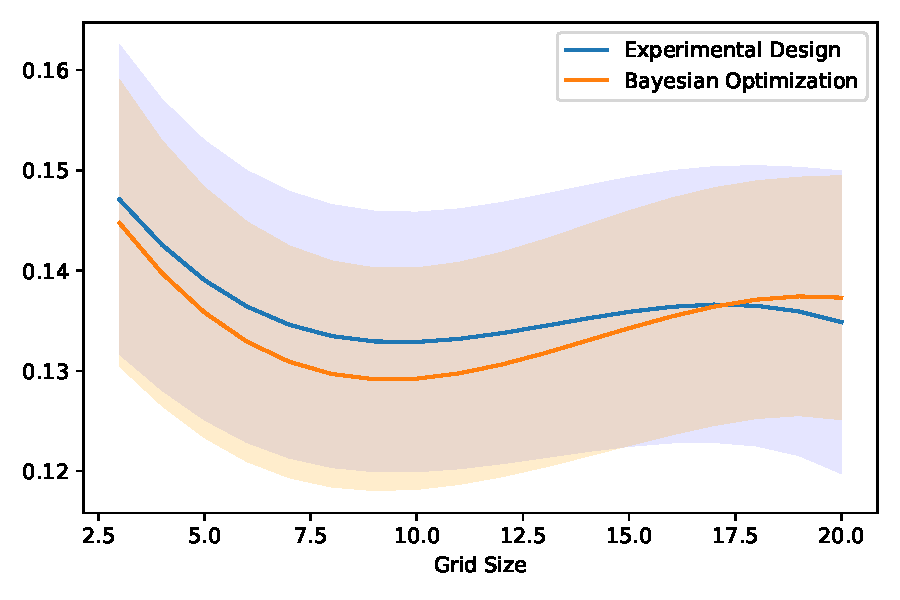
\includegraphics[width=\textwidth]{images/ofat_compare/time/grid_size.pdf}
  \caption{Time loss}
\end{subfigure}%
\begin{subfigure}{0.5\textwidth}
  \centering
  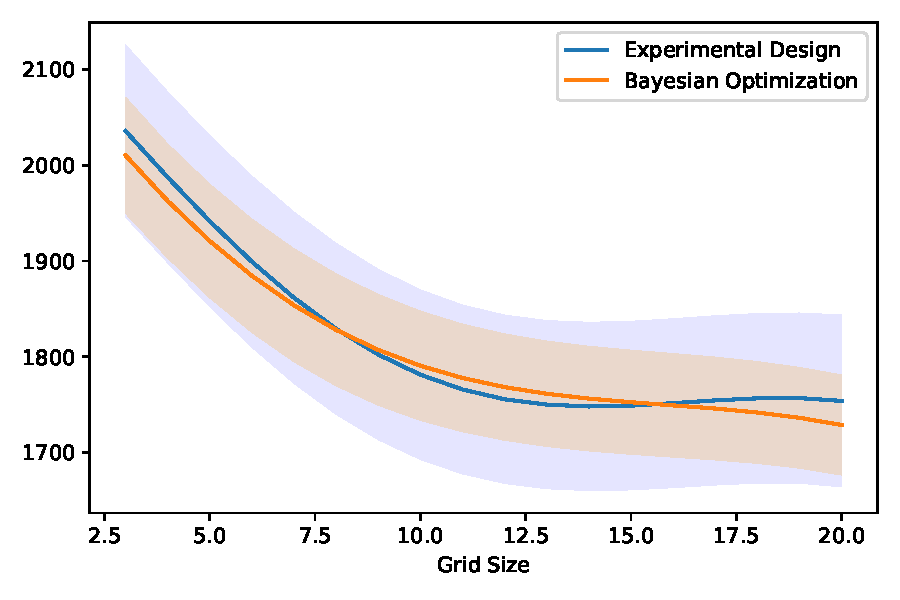
\includegraphics[width=\textwidth]{images/ofat_compare/co2/grid_size.pdf}
  \caption{CO$_2$}
\end{subfigure}
\caption{Experimental design and Bayesian Optimisation model comparison for grid size in the average optimal point}
\label{fig:grid_size_comp}
\end{figure}
